\documentclass[tikz,border=5pt]{standalone}
\usepackage{newtx}
\newcommand*{\drawellipse}[2]{%
    \draw[dashed,thick] #1 arc[start angle=180, end angle=0,x radius=#2cm, y radius=\fpeval{(#2/4)}cm];
    \draw[thick] #1 arc[start angle=180, end angle=360,x radius=#2cm, y radius=\fpeval{(#2/4)}cm];
}
\begin{document}
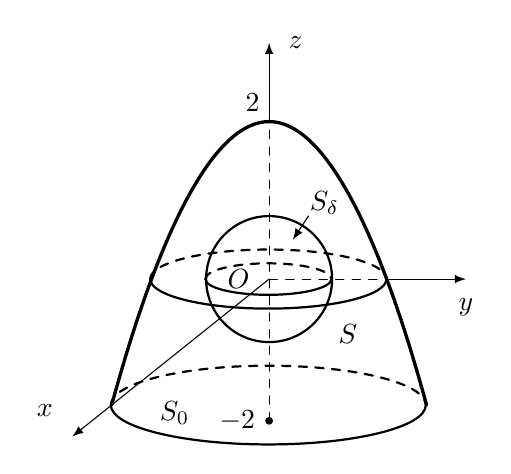
\begin{tikzpicture}[line cap=round,line join=round]
    \draw[dashed] (0,-1.8) -- (0,2) coordinate (z0);
    \node[label=left:{$-2$},shape=circle,fill,inner sep=1pt] at (0,-1.8) {};
    \draw[dashed] (0,0) coordinate (O)  -- (1.5,0) coordinate (y0) ;
    \draw[-latex] (O) node[label=left:$O$] {} -- (-2.5,-2) coordinate (x0) node[label= above left:{$x$}] {};
    \draw[-latex] (y0) -- ++(1,0) node[label=below:{$y$}] {};
    \draw[-latex] (z0) -- ++(0,1) node[label=right:{$z$}] {};
    \draw[very thick] (-2,-1.6) parabola[parabola height=3.6cm] +(4,0);
    \drawellipse{(-1.51,0)}{1.5}
    \drawellipse{(-2.01,-1.6)}{2}
    \draw[thick] circle [radius=.8cm];
    \drawellipse{(-.81,0)}{.8}
    \draw node[above left] at (z0) {$2$} node at (-1.2,-1.7) {$S_0$} node at (1,-.7) {$S$};
    \draw[-latex] (.5,.8) node[above right=-3pt] {$S_\delta$} -- ++(-.2,-.3);
\end{tikzpicture}
\end{document}


